\documentclass[a4paper,11pt,titlepage]{report}

%Per gli accenti%
\usepackage{amsmath,latexsym}
\usepackage[T1]{fontenc}
\usepackage[utf8]{inputenc} %modo di scrittura del file
\usepackage[italian, english]{babel} %accenti
\usepackage{amsthm, amstext} %per i teoremi
\usepackage{geometry} %modificare le dim della pagina
\usepackage{graphicx} %modificare immagine
\usepackage{tabularx} % " tabelle
\usepackage{multicol} % scrivere in più colonne
\usepackage{subfigure}
\usepackage{mathtools}
\usepackage{color}
\usepackage{verbatim} %commentare \begin{comment}
\usepackage{hyperref}
\usepackage{amssymb, mathrsfs}
\usepackage{amsfonts}
\usepackage{verbatim} %commenti
%\graphicspath{ {C:\Users\MalcomIII\Desktop\Università\Fisica\III My\Tesi\Tesi Benettin\Tesi} }
\usepackage{enumitem} % elenco puntato 
\SetLabelAlign{parright}{\parbox[t]{\labelwidth}{\raggedleft#1}}
\setlist[description]{style=multiline,leftmargin=0.3cm, align=parright,noitemsep}


%introdurre def
\theoremstyle{definition} 	
\newtheorem{defn}{Definizione}[chapter] 
%introdurre prop
\theoremstyle{plain}
\newtheorem{prop}{Proposizione}
%introdurre corollario
\newtheorem{cor}{Corollario}

\DeclarePairedDelimiter\bra{\langle}{\rvert}
\DeclarePairedDelimiter\ket{\lvert}{\rangle}
\DeclarePairedDelimiterX\braket[2]{\langle}{\rangle}{#1 \delimsize\vert #2}

\usepackage{etoolbox}
\patchcmd{\thebibliography}{\section*{\bibname}}{\Large{\textbf{Bibliography}}}{}{}
\patchcmd{\thebibliography}{\section*{\refname}}{\Large{\textbf{Bibliography}}}{}{}

\setlength\parindent{0pt}



\makeatletter

\newcommand\frontmatter{%
	\cleardoublepage
	%\@mainmatterfalse
	\pagenumbering{arabic}}

\newcommand\mainmatter{%
	\cleardoublepage
	% \@mainmattertrue
	\pagenumbering{arabic}}

\newcommand\backmatter{%
	\if@openright
	\cleardoublepage
	\else
	\clearpage
	\fi
	%\@mainmatterfalse
}

\makeatother

\usepackage{fancyhdr} 
\setlength{\headheight}{15pt}

\pagestyle{fancy}

\begin{document}
	
\fancyhf{}
\fancyhead[LE,RO]{\thepage}
\fancyhead[RE]{\textit{ \nouppercase{\leftmark}} }
\fancyhead[LO]{\textit{ \nouppercase{\rightmark}} }


\frontmatter

\newgeometry{left=2.5cm,right=2.5cm, top=2cm, bottom=2cm}

\begin{titlepage}
\begin{center}
\begin{figure}
\centering

\includegraphics[scale=0.3]{logo.png}
\end{figure}
\large\textbf{ {Università degli studi di Padova}}\\
\vspace{6em}
\Large{Dipartimento di Fisica e Astronomia "Galileo Galilei"}\\
\vspace{2em}
\Large{Dipartimento di Matematica "Tullio Levi-Civita"}\\
\vspace{2em}
\large{Corso di Laurea Triennale in Fisica}\\
\vspace{5em}
\large{Tesi di Laurea}\\
\LARGE{\textbf{La stabilità dei punti lagrangiani L4 e L5: sviluppi recenti}}\\
\vspace{5em}
\end{center}
\Large\textbf{{Laureando: }}\hspace{1.5em}\Large{Riccardo Milocco}\\

\Large\textbf{{Relatore: }}\hspace{1.2em}\Large{Prof. Giancarlo Benettin}\\
%\Large\textbf{{Correlatore: }}\hspace{1.2em}\Large{Prof. ****}\\
\vspace{4em}
\begin{center}
\large{Anno accademico 2016-2017}
\end{center}
\end{titlepage}

\restoregeometry

\newpage
\thispagestyle{empty}
\mbox{}


\newpage
\thispagestyle{empty}

\selectlanguage {italian}
\tableofcontents
\chapter*{Introduzione}

In meccanica classica date le equazioni di Newton e il principio di unicità di Cauchy, si può determinare univocamente la dinamica del sistema preso in esame.
Queste equazioni, in realtà, lasciano definita l'orbita descritta dal sistema tramite delle equazioni differenziali del secondo ordine che, in generale, non sono integrabili.
Consideriamo, infatti un modello elementare di \textit{n} corpi in interazione attraverso la forza gravitazionale. Ad oggi, solo per $\textit{n} \leq 2$ troviamo un soluzione esplicita del problema. Se passiamo a $\textit{n}=3$ Poincarè e Burns hanno dimostrato, alla fine del XIX secolo, che non esiste alcuna soluzione analitica del problema.
Per $n=3$, il problema è con evidenza definito \textit{Problema dei tre corpi}.
In questo lavoro di tesi, illustreremo i recenti sviluppi relativi allo studio della stabilità degli equilibri di un caso particolare di questo problema: il \textit{Problema dei tre corpi ristretto circolare piano}.
In particolare, analizzaremo in ambito hamiltoniano il modello composto da Sole-Giove (i "primari") e gli asteroidi Troiani.
\\Si assume, inoltre, che il modello sia \textit{"ristretto"}, in quanto il moto degli asteriodi non influisce sul moto dei primari; \textit{"circolare"}, poichè il moto dei primari, rispetto al baricentro del sistema, è circolare e non ellittico; e \textit{"piano"}, perchè si analizza la dinamica dei Troiani ristretta al piano del moto dei due primari.
Ricordiamo che il problema a tre corpi ha cinque punti di equilibrio detti punti lagrangiani: tre stanno sulla direttrice dei due corpi principali (i "primari"); mentre L4 \textit{(risp. L5)} giace sul terzo vertice superiore \textit{(risp. inferiore)} del triangolo equilatero che ha come altri vertici i due primari (vedi \ref{fig:Lagr}). Per la loro posizione rispetto ai primari, i primi tre sono detti "collineari" e L4,L5 sono chiamati "punti triangolari".\\
In questa tesi, esporremo dei metodi analitici per determinare il dominio di stabilità per tempi arbitrariamente grandi in prossimità di L4. \\Si noti che L5 ha una trattazione del tutto equivalente a quella sviluppata per L4. Pertanto, tratteremo solo il caso di L4.\\\\
Per quanto riguarda la stabilità dei punti lagrangiani, si dimostra che, attraverso il teorema spettrale di Lyapunov, i punti "collineari" L1,L2,L3 sono instabili; mentre per L4 e L5 la trattazione è più complessa.
\\Anche se verrà trattato con più attenzione nelle sezioni seguenti, è bene già rendere evidente qual è il limite principale del metodo analitico utilizzato finora. 
\\Preliminarmente, ci poniamo in coordinate polari in un sistema di riferimento con l'origine su L4. Secondariamente, espandiamo in serie di Taylor l'hamiltoniana e applichiamo il già citato teorema di Lyapunov all'hamiltoniana linearizzata.
Definito il parametro\footnote{$m_J, M_S$ sono, rispettivamente, la massa di Giove e del Sole} $$\mu:= \frac{m_J}{m_J+M_S},$$ si trova che i punti "triangolari" per il sistema completo sono
\begin{itemize}
	\item instabili per il sistema completo per $ \mu \geq 1-\mu_R$ \\( con $\mu_R\simeq0.0038$ \textit{"limite di Routh"});
	\item altrimenti, la stabilità non è garantita per ogni orbita.
\end{itemize}
In particolare, troveremo che l'hamiltoniana linearizzata non ha un minimo stretto nell'origine. Pertanto, sarà di vitale importanza valutare la dinamica delle orbite data dai termini successivi dell'espansione dell'hamiltoniana completa. Ricordiamo che se l'hamiltoniana avesse un punto di minimo stretto nell'origine, allora grazie al \textit{teorema di Lagrange-Dirichlet} potremo concludere che la stabilità di L4 è garantita anche con l'aggiunta dei termini d'ordine superiore che formano ò'hamiltoniana completa.
Tuttavia, si osservano sperimentalmente due insiemi di asteroidi, detti "Troiani" e "Greci", che giacciono rispettivamente su L4 e L5. Il problema di stabilità è, dunque, di natura analitica. Difatti, non si possiedo ancora gli opportuni strumenti matematici per dimostrare la stabilità di ogni orbita nell'intorno di L4 (L5) per un tempo arbitrariamente grande. Dunque nonstante i rilevanti successi ottenuti di recente, la stabilità di L4-L5 è ancor oggi oggetto di ricerca scientifica.

\begin{figure}[h]
	\centering
	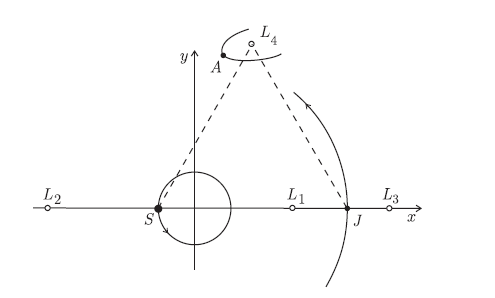
\includegraphics[scale=0.8]{PuntiLagrangiani.png}
	\label{fig:Lagr}
	\caption{I punti di equilibrio lagrangiani nel problema ristretto a tre corpi}
\end{figure}
L'obiettivo, dunque, sarà quello di considerare il problema di stabilità di L4, nello spirito della teoria di stabilità di Nekhoroshev, per lunghi intervalli di tempo. Per la precisione, si stimerà la regione dello spazio dove è assicurata la stabilità delle orbite per ordini di tempo dell'età dell'universo.

\chapter{Metodo Analitico}
Per prima cosa trovata l'hamiltoniana del problema, si è offrontato il problema della stabilità del punto L4 in un preciso intorno nel quale il sistema è linearizzabile. Tuttavia passando alle coordinate normali, si nota che il sistema linearizzato è formato da due oscillatori armonici disaccoppiati di cui uno a frequenza negativa. \textcolor{red}{Quest'ultima condizione, di trascurabile significato per il sistema linearizzato, fa sì che l'hamiltoniana del sistema non abbia un punto di minimo in L4.
Pertanto, come vedremo meglio nella sezione 2.3, non si può concludere che l'aggiunta di termini successivi non infici la stabilità del punto.
Sarà indispensabile valutare in che modo i termini di ordine superiore agiscano sulla dinamica del sistema.}

Come riportato in \cite{OTSA}, illustriamo ulteriori metodi per ottenere delle stime di stabilità.
\\\\Il primo riguarda l'individuazione di due integrali primi che sono anche costanti del moto: le azioni. Pertanto, si pone l'hamiltoniana in forma normale, come previsto dal metodo indiretto di Birkhoff. In questo modo, le azioni nelle coordinate normali sono (quasi) esattamente delle costanti del moto nel dominio di stabilità fissato. 
\\Il secondo riguarda la definizione di una famiglia di domini di stabilità e una buona norma per stimare la grandezza delle funzioni in gioco (ad. es. la scala di tempo in cui evolvono le azioni \(\dot{I}\) ). \\Nel dettaglio useremo le coordinate polari per descrivere il dominio di stabilità.  
Infatti, da un'analisi numerica si può notare che la proiezione della regione di stabilità sul piano dei primari è, in prima approssimazione, un'ellisse con centro in L4 ( vedi \cite{1989}).
\begin{figure}[h]
	\label{fig:Ellisse}
	\centering
	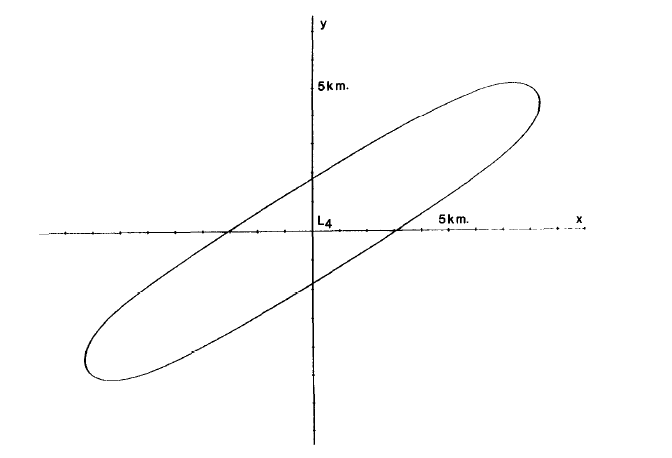
\includegraphics[scale=0.8]{Ellisse.png}
	\caption{Proiezione sul piano cartesiano $(x,y)$ del dominio di stabilità di L4 nel modello Sole-Giove senza risonanze\cite{1989}} 
\end{figure}
\\Per quanto riguarda l'introduzione della norma, rimandiamo la spiegazione all'apposita sezione.
\\\\Il terzo riguarda il calcolo del minimo "tempo di fuga", ovvero il minimo intervallo temporale impiegato da un'orbita per uscire dal dominio di stabilità. 
Grazie a questa stima otterremo, inoltre, il miglior ordine di espansione dell'hamiltoniana. 
Infatti dalla teoria di Nekhoroshev, l' espansione in serie che deriva dalla teoria delle perturbazioni classica ha un carattere asintotico. Pertanto, esiste un valore ottimale tale che il "resto" sia trascurabile.  
\\\\Infine, si confronteranno i risultati ottenuti con l'effettiva regione di stabilità osservata.

\chapter {Contesto teorico}
Nella sezione I di questo capitolo si procede con l'introduzione dell'hamiltoniana per il problema a tre corpi circolare piano.
\\Nella sezione II si troveranno i punti di equilibrio del sistema.
\\Nella sezione III si analizzerà la natura del punto lagrangiano L4.

\section {Problema ristretto circolare piano}

Consideriamo un sistema di riferimento corotante con i primari $ (0,q_1,q_2) $, l'origine situata sul centro di massa del sistema Sole-Giove e l'asse delle ascisse $ q_1 $ posto sulla direttrice dei due pianeti orientata verso il Sole.
\textcolor{red}{Si assumono, inoltre, unità di misura tali che, denotata $$\mu = \frac{m}{m+M}  ,$$ la distanza tra i pianeti sia 1, la velocità\footnote{$\omega \in \mathbb{R}^3$ t.c. $\omega^2a^3 = G(M+m)$} $\omega$ di rotazione di Giove sia unitaria, la massa complessiva del sistema sia 1 e la costante gravitazionale $\mathcal{G}$ sia unitaria. Dunque, il Sole avrà massa $ 1-\mu $ e giacerà sempre sul punto $(\mu,0)$; mentre Giove avrà massa $ \mu $ e si troverà in $ (1-\mu,0) $.}
\\L'hamiltoniana per un asteroide avrà la forma

\begin{equation}
\label{hamiltoniana1}
H = \frac{1}{2} ( p_1^2 + p_2^2) + q_2p_1 - q_1p_2 - \frac{1- \mu}{\sqrt{( q_1 - \mu )^2 +q_2^2 }} - \frac{\mu}{\sqrt{( q_1 + 1 - \mu )^2 +q_2^2 )}}
\end{equation}

\section {Punti di equilibrio lagrangiani}

Ponendo uguale a zero ogni derivata parziale di $H$ si ha
$$p_3=0, \quad q_3=0,\quad p_1=-q_2,\quad p_2=q_1,$$ 
\begin{equation} 
\label{eq:Plagr1}
q_2(-1+ \frac{(1-\mu)}{R^{3}} + \frac{\mu}{r^{3}} )  
\end{equation}
\begin{equation} 
\label{eq:Plagr2}
-q_1 + \frac{(1-\mu)(q_1+\mu)}{R^{3}} + \frac{\mu (q_1-q+\mu)}{r^{3}} \end{equation}
\\\\Risolvendo le \ref{eq:Plagr1} e \ref{eq:Plagr2}, rispetto a $q_1$ e $q_2$, si ottengo i punti d'equilibrio o punti "lagrangiani": posto $q_2=0$ nella \ref{eq:Plagr2} otteniamo $L_1$,$L_2$,$L_3$ detti "collineari"; mentre con $q_2\neq0$ e $R=r$ si determinano $L4$ e $L5$ detti "triangolari". Quest'ultimi, infatti, giacciono rispettivamente sul vertice superiore e inferiore dei due triangoli equilateri speculari \textcolor{red}{rispetto alla base comune Sole-Giove.}
In conclusione come illustrato in \ref{fig:Lagr} ???FIGURA 1, L4 è individuato da $$ q_1 = - \frac{(1- 2\mu)}{2}, \quad q_2 = - \frac{\sqrt{3}}{2}, \quad p_1 = - q_2, \quad p_2 = q_1 $$
\section{Verso l'hamiltoniana in forma normale}

Per essere trattata con il metodo di Birkhoff, l'hamiltoniana deve presentare delle determinate caratteristiche. Dunque, si trasforma la \ref{hamiltoniana1} con una serie di funzioni generatrici di trasformazioni canoniche riportate in \cite{OTSA}:
\\\\1) trasliamo l'origine sul Sole (modello eliocentrico) grazie alla trasformazione di coordinate $\mathcal{T}$ tale che $$\mathcal{T} := 
\begin{cases}
	\quad Q_1 =q_1 -\mu   \\
	\quad Q_2 =q_2  \\
	\quad P_1 =p_1  \\
	\quad P_2 = p_2 - \mu 
\end{cases} 
$$
\\dove $ Q_1 $ , $ Q_2 $ , $ P_1 $, $ P_2 $ sono le nuove coordinate eliocentriche.

Osserviamo che la trasformazione $\mathcal{T}$ può essere ottenuta dalla generatrice $$ W_1(p_1, p_2, Q_1, Q_2) = -(Q_1+ \mu)p_1 - Q_2(p_2- \mu). $$
Infatti si dimostra che, derivando l'opposto della nostra funzione generatrice ($-W_1 $) rispetto alle variabili, ricaviamo la $\mathcal{T}$ a meno di una immediata inversione.     
Per l'appunto si trova che 
$$\begin{cases}
\quad q_1 = Q_1 + \mu    \\
\quad q_2 = Q_2 \\
\quad P_1 = p_1  \\
\quad P_2 = p_2 -\mu 
\end{cases} $$
\\2) eseguiamo un cambio alle coordinate polari con $\mathcal{P}$ tale che
$$ \mathcal{P} :=\begin{cases}
\quad \rho= \sqrt{Q_1^2 + Q_2^2}    \\
\quad \theta= \tan(\frac{Q_2}{Q_1}) \qquad \hbox{se } Q_1 > 0,\quad Q_2 \geq 0\\
\quad p_{\rho} = \frac{P_1Q_1+P_2Q_2}{\sqrt{Q_1^2 + Q_2^2}}\\
\quad p_{\theta} = P_2Q_1-P_1Q_2
\end{cases} $$ 
\\dove $ \rho $ , $ \theta $ , $ p_\rho $, $ p_\theta $ sono le nuove coordinate polari. Notiamo che $p_{\rho}$ è, con evidenza, il momento angolare di un punto che si muove di moto circolare sul piano $(x,y)$.
La suddetta trasformazione è stata ricavata, applicando il metodo esposto precedente alla $$ W_2 = -\rho(P_1 \cos(\theta) + P_2\sin(\theta) ). $$
Quindi, $$\begin{cases}
	\quad p_\rho= P_1\cos(\theta)+P_2\sin(\theta)    \\
	\quad p_\theta= \rho(P_2 \cos(\theta)-P_1\sin(\theta))\\
	\quad Q_1 = \rho \cos(\theta)  \\
	\quad Q_2 = \rho \sin(\theta)
\end{cases} $$
\\3) Considerando $ \theta $ come una coordinata non periodica, introduciamo un sistema di riferimento nell'intorno di L4. Ricordando che in queste coordinate L4 è individuato da $ \rho = 1 $ , $ \theta = \frac{2\pi}{3} $ , $ p_\rho = 0 $, $ p_\theta = 1 $ , si trasla l'origine sul punto in questione con $\mathcal{T'}$ tale che $$\mathcal{T'} := 
\begin{cases}
\quad x = \rho -1\\
\quad y =\theta -2\pi/3  \\
\quad p_x =p_{\rho}  \\
\quad p_y = p_{\theta}-1 
\end{cases} 
$$
\\dove $ x $ , $ y $ , $ p_x $, $ p_y $ sono le nuove coordinate canoniche.
Come prima, la $\mathcal{T'}$ si ottiene dalla $W_3$  $$ W_3 = p_x(\rho - 1) + (p_y+1)\theta - \frac{2\pi}{3} p_y $$ 
\\Dalla figura sottostante, diventa chiaro perchè abbiamo utilizzato questo complicato procedimento. Infatti, le nuove coordinate si adattano bene alla descrizione dell'orbita percorsa da un asteroide troiano nei pressi di L4.
(INSERIRE FIGURA)

Date le coordinate $ x $ , $ y $ , $ p_x $, $ p_y $, l'hamiltoniana assumerà la forma
$$ H = \frac{1}{2} [ p_x^2 + (\frac{p_y+1}{x+1})^2] -p_y - \mu (x+1)\cos( y + \frac{2\pi}{3} ) - \frac{1- \mu}{1+x} - \frac{\mu}{\sqrt{( x+1 )^2+1+2(x+1)\cos(y+\frac{2\pi}{3})}} $$


4) Si espande l'hamiltoniana in serie di Taylor in un intorno dell'origine, ottenendo uno sviluppo della forma $ H = H_2 + H_3 + H_4 +\dots $
\\dove $$ H_2 = \frac{1}{2} ( p_x^2 + p_y^2) - 2xp_y + ( \frac{1}{2} + \frac{9\mu}{8})x^2 - \frac{9\mu}{8}y^2 + \frac{3 \sqrt{3 \mu}}{4} xy) $$
\\e $ H_s $ per $ s > 2 $ è un polinomio omogeneo di grado s nelle varibili canoniche.
Avendo trovato la forma della linearizzata $H_2$, ne calcoliamo gli autovalori per dare una stima della stabilità del punto.\\
Notando che $H_2$ è reale, si sa che se $\lambda$ è autovalore di $H_2$ lo sarà anche $\bar{\lambda}$. In più dato che è simplettica, si trova anche la coppia di autovalori $-\lambda$, $-\bar{\lambda}$.
\\Dunque se tutti gli autovalori sono immaginari puri, il punto sarà stabile, o anche detto "ellittico"; mentre se almeno un autovalore avrà parte reale negativa, il punto sarà instabile, o "iperbolico".
Nel dettaglio, si trova che, definito $$ \mu_R = \frac{1}{2} ( 1- \sqrt{\frac{23}{27}}) \simeq 0.0385 $$  ("limite di Routh"): 
\begin{itemize}
	\item se $\mu \leq \mu_R \quad (1-\mu) \leq \mu_R$ allora l'equilibrio è "ellittico";
	\item altrimenti è "iperbolico".
\end{itemize}
5) Per la teoria delle piccole oscillazzioni, in un intorno dell'equilibrio ellittico possiamo introdurre delle coordinate normali tali che la $H_2$, sia composta da due oscillatori armonici disaccoppiati. \\Dunque per $\mu \leq \mu_R$ e applicando le nuove coordinate (cartesiane) normali ($ x_1 $ , $ y_1 $ , $ x_2 $, $ y_2 $), \\$H_2$ assumerà la forma diagonale $$H_2 = \frac{\omega_1 (x_1^2+y_1^2)}{2} -\frac{\omega_2 (x_2^2+y_2^2)}{2} \quad \omega_1 > 0 , \quad \omega_2 < 0 $$
\\dove $ \omega_1 $, $ \omega_2 $ le frequenze di oscillazione rispetto a L4.

Osserviamo che l'hamiltoniana precedente rappresenta due oscillatori armonici disaccoppiati e, dunque in prima approssimazione, si ritrovano le orbite circolari illustrate in \ref{fig:Ellisse}.

Come riportato in \cite{OTSA}, la trasformazione alle coordinate normali è lineare e data dalla matrice simplettica\\
$$ C = ( e_1m_1^{-\frac{1}{2}}, e_2m_2^{-\frac{1}{2}}, f_1m_1^{-\frac{1}{2}} , f_2m_2^{-\frac{1}{2}} ) $$
\\dove i vettori colonna reali sono dati dalla $$ e_j + if_j= \left( \begin{array}{llcl}
\frac{8 \omega_j^2 + 4 \sqrt{3} \alpha +9}{8} \\ \frac{16i \omega_j+4 \alpha +3 \sqrt{3}}{8} \\ i \omega_j \frac{8 \omega_j^2 + 4 \sqrt{3} \alpha}{8} \\ i \omega_j \frac{4 \alpha +3\sqrt{3}}{8} + \frac{4\alpha\sqrt{3}+9}{4}
\end{array}\right)$$
\\e costanti $m_j (j=1,2)$ date dalla $m_j=\omega_j D_j$, 
$$ D_j = ( \frac{8\omega_j^2 + 4 \sqrt{3}\alpha}{8})^2 - 2 (\sqrt{3}\alpha + \frac{9}{4} ) + (\frac{4\alpha+3\sqrt{3}}{8})^2$$ \\ e $\omega_1^2$, $\omega_2^2$, $\alpha$ sono definite come $$ \omega_1^2 = \frac{1}{2} + \frac{1}{2} \sqrt{1 - \frac{27}{4} + 4\alpha^2}, \quad  \omega_2^2 = \frac{1}{2} - \frac{1}{2} \sqrt{1 - \frac{27}{4} + 4\alpha^2}, \quad \alpha = - \frac{(1-2\mu)e\sqrt{3}}{4} $$
\textcolor{red}{Si noti che per avere $m_j > 0$, condizione necessaria perchè $C$ sia simplettica, basta imporre che $\omega_1 > 0$ , $\omega_2 < 0$. Quest' ultima condizione fa sì che l'origine non sia più un punto di minimo assoluto per l'hamiltoniana $H$ del sistema completo: precisamente L4 è punto di sella e non si può applicare il \textit{teorema di Lagrange-Dirichlet} per dimostrare la stabilità. Quindi, a differenza del sistema linearizzato, l'aggiunta di termini di $O(q^3)$ sarà fondamentale per determinare la natura del punto sotto la dinamica di H}.

\chapter{Studio della stabilità di L4}
In questo capitolo, riportiamo il metodo analitico di \cite{OTSA} per ottenere delle stime di stabilità di L4. Infatti,  l'analisi condotta fino ad ora è risultata insoddisfacente.
\\\\Nella prima sezione si pone l'hamiltoniana nella forma normale di Birkhoff per trovare due integrali del moto.
\\Nelle sezioni II, III si studiano, rispettivamente, il dominio di stabilità nonchè l'introduzione di una buona norma; e, "valutando il tempo di fuga", il miglior ordine di espansione dell'hamiltoniana perturbata.
\\Infine nella sezione IV, si analizzano i risultati ottenuti con i dati sperimentali. 

\section {Costruzione della forma normale}

\subsection{Metodo di Birkhoff}

In questa parte, richiameremo i punti salienti della costruzione normale di Birkhoff, per poi applicarla al nostro problema. Scopo di questa manipolazione è trovare una forma dell'hamiltoniana che, in  condizioni di non risonanza per le frequenze $\omega:=(\omega_1,\omega_2)$ di $H_2$, permetta di determinare facilmente delle costanti del moto.
In particolare, dobbiamo risolvere l'equazione $\{H,\varPhi\} = 0$, dove $\varPhi$ sono gli integrali del moto. 
\\Per rendere il calcolo più diretto, agiremo sull'hamiltoniana di partenza $H$ per portarla nella cosiddetta \textit{"forma normale di Birkhoof $H^{(r)}$"}. 
\\Precisamente, $H^{(r)}$ è \textit{"in forma normale di Birkhoof (all'ordine r)"} se assume lo svillupo $$H^{(r)} = H_2 + Z_3+ Z_4 + \dots+ Z_r + \mathcal{R}^{(r+1)} $$ \\dove $H_2$ è diagonale, $Z_r$ dipende solo delle azioni $I_j$ con $Z_r = I_j^r= (\frac{x_j^2+y_j^2}{2})^r $ e $ \mathcal{R}^{(r+1)} $ è il "resto": lo sviluppo successivo della serie partendo dall'ordine r+1. Siccome il resto non è in forma normale, esso sarà una combinazione \textcolor{red}{delle diverse azioni $I_j$}.
Data $H^{(r)}$ e ricordando che $\{I_j, F(I_j)\} = 0$ per ogni $F reale?????????$, osserviamo che le costanti del moto cercate sono proprio le azioni\footnote{Precisamente indicate con $(x,y)$ e $(x',y')$ le coordinate prima e dopo la costruzione della forma normale, le azioni sono integrali primi per il sistema in forma normale, $\{H^{(r)}(x',y'),I_j(x',y')\}=0$. Inoltre, le azioni continueranno ad essere integrali primi di $H(x,y)$ ma nelle vecchie coordinate $(x,y)$.} $I_j$ con $j=1,2$.
 
\subsection{Operatore di Lie}
Identificato l'obbiettivo, abbiamo bisogno di introdurre l' operatore $T_{\chi}$, detto \textit{"opertaore di Lie"}, che ci permetterà di trovare la forma normale $H^{(r)}$ fino all'ordine r.
\begin{defn}
	\label{defT}
	Sia $ \varPi $ lo spazio vettoriale dei polinomi omogenei, definiamo la successione di polinomi omogenei di gradi $s$ come $\chi:= \{\chi_s\}_{s\geq3} $ , con $ \chi_s \in \varPi $. \\Definiamo, inoltre, $E \in \varPi$ con $E:\varPi \longrightarrow \mathbb{R}$ e $T_\chi :\varPi \longrightarrow \varPi $ \textit{"operatore di Lie"} tale che
	$$ T_\chi E = \sum_{s\geq0} E_s $$
	$$E_0=1, \qquad E_s = \sum_{j=1}^{s} \frac{j}{s} \textit{L}_{\chi_{j + 2}}E_{s-j} $$ 
	dove $\textit{L}_{\chi} * = \{\chi, *\}$ è la derivata di Lie di $*$ rispetto a $\chi_s$ detta "hamiltoniana generatrice della forma normale (fino) all'ordine s"  
\end{defn}

\begin{prop}
Come riportato in \cite{1977}, l'operatore $T_\chi$ definito nella \ref{defT} ha le seguenti proprietà:
	\begin{enumerate}
		\item è lineare, ovvero $T_\chi(\alpha v+ \beta w)= \alpha T_\chi v+\beta T_\chi w$, dove $\alpha$, $\beta$ sono numeri reali e $v$,$w$ possono essere sia funzioni reali che campi vettoriali; 
		\item conserva il prodotto, ossia $T_\chi (f \cdot g) = T_\chi f \cdot T_\chi g$, ove $f$,$g$ sono funzioni;
		\item preserva le parentesi di Poisson tra campi vettoriali: $\{T_\chi{v,w}\} = \{T_\chi v,T_\chi w\}$ \\con $v$,$w$ campi vettoriali;
		\item invertibile: $$T_{\chi}^{-1} := \sum_{j=1}^{s} G_s$$
		$$ G_0=E_0 \qquad G_s = - \sum_{j=1}^{s} \frac{j}{s}G_{s-j} \textit{L}_{\chi_j}$$	
	\end{enumerate}	
\end{prop}

\begin{cor}
 Data la conservazione delle parentesi di Poisson\cite{1977}, $T_\chi$ genera una\\     trasformazione alle nuove coordinate canoniche $(x',y') \in \varPi$ della forma
	\begin{equation}
		\label{cambiodicoor}
		x' = T_{\chi^{(r)}} x, \quad y' = T_{\chi^{(r)}} y
	\end{equation}
\end{cor}
\begin{cor}
	Sia $f$ come sopra e $(x,y)$,$(x',y')$ rispettivamente le nuove e vecchie\\ coordinate, allora
	\begin{equation}
	\label{[proprietàT]}
	f(x,y)|_{(x,y)=T_{\chi}^{-1}(x',y')} = (T_{\chi}^{-1}f)(x',y')  \qquad \hbox{per} \hspace{2mm} (x',y'),(x,y),f\in \varPi
	\end{equation}
\end{cor}		

\subsection{Applicazione del metodo di Birkhoff}
Definito $T_\chi$, possiamo ora verificare che se $H^{(r)}$ è l'hamiltoniana in forma normale e $H$ l'hamiltoniana di partenza allora 
\begin{equation}
\label{eq:fndbirk}
T_{\chi^{(r)}} H^{(r)} = H
\end{equation} 
Il problema ora è trovare le successioni $\{\chi_s\}_s$ e $\{Z_s\}_s$ ($s \in [3,r]$) tali che sia soddisfatta la \ref{eq:fndbirk}.
Tuttavia per $\omega$ non risonanti, $\chi_s$ e $Z_s$ si determinano contemporaneamente, risolvendo l'equazione \ref{eq:fndbirk} rispetto alle incognite $\chi_s$ e $Z_s$.

Preliminarmente ricordando la definizione \ref{defT} e esplicitando la \ref{eq:fndbirk}, $$ \sum_{s\geq3} E_s (H_2+Z_3+\dots+Z_r+\mathcal{R}^{(r)}) = H_2+H_3+\dots $$
\\Osserviamo che $E_s$ contiene la successione $\{\chi_3,\dots,\chi_{s+2}\}$ e data $g$ è di ordine r, allora $E_s \hspace*{0.5mm} g$, tenendo conto dell'azione della parentesi di Poisson, è di ordine $s+r$.
\\Uguagliando ora ogni ordine nell'equazione precedente, generiamo una famiglia di equazioni che si risolvono in maniera "gerarchica\footnote{Una rappresentazione grafica dello schema risolutivo è riportata in appendice.}".
Infatti dall'osservazione precedente e definendo $Z_{s-k}^k:= E_k\hspace{0.5mm}Z_{s-k}$, otteniamo$$
\begin{cases}
	\quad Z_2=H_2 \\
	\quad Z_s = H_s - \sum_{k=1}^{s-2} Z_{s-k}^{k} \quad $s=3,\dots,r$
\end{cases}
$$
Notiamo che dalle equazioni precedenti si nota che $f_{s-2}$ contiene le hamiltoniane generatrici $\{\chi_3,\dots,\chi_s\}$ ed è l'unico termine con $\chi_s$.
Pertanto, il sistema precedente si può scrivere nella forma 
$$ Z_s - \mathcal{L}_{H_2}\chi_s = H_s + Q_s \qquad s= 2,\dots,r$$
\\ove $\mathcal{L}_{H_2} \hspace{0.5mm} *=\{H_2,*\}$ e $Q_s$ è un polinomio di ordine s, dipendente da $\chi_t$ e $Z_t$ con $t=1,\dots,s-1$.
\\Detto, quindi, $P_s^{(s-1)}:= H_s + Q_s$ il polinomio di ordine $s$ totalmente determinato dagli $s-1$ passi precedenti, osserviamo che 
\begin{equation}
	\label{eq:eqbirkFACILE} 
	\mathcal{L}_{H_2}\chi_s =  Z_s - P_s^{(s-1)}
\end{equation} e ora, avendo già ottenuto ai passi precedenti le variabili all'ordine $s-1$, riusciamo a determinare $\chi_s$ e $Z_s$.
\\A questo punto sviluppando la derivata di Lie della \ref{eq:eqbirkFACILE} nelle variabili cartesiane $(x_1,x_2)$ e momenti coniugati $(y_1,y_2)$, troviamo che la \ref{eq:eqbirkFACILE} non è risolvibile.
Per ovviare al problema, applichiamo una trasformazione alle coordinate
($\xi_j$, $\eta_j$ ) (per $j=1,2$) della forma \\
\begin{equation}
	\label{eq:cambiodv}
	x_j= \frac{1}{\sqrt{2}} ( \xi_j + i \eta_j), \qquad y_j= \frac{1}{\sqrt{2}} ( \xi_j - i \eta_j), \qquad \hbox{per} \hspace{2mm} j=1,2
\end{equation}
	\\\\con inversa 
	$$ \xi_j = \frac{1}{\sqrt{2}} (x_j-iy_j), \qquad 
		\eta_j = \frac{1}{\sqrt{2}} (\frac{x_j}{i}+y_j), \qquad \hbox{per} \hspace{2mm} j=1,2. $$
\\Osserviamo che nelle nuove coordinate $$H_2 = i( \omega_1 \xi_1\eta_1+\omega_2\xi_2\eta_2);$$ mentre le azioni $$I_j(\xi_j,\eta_j)=i\omega_j \eta_j \xi_j \qquad \hbox{con} \quad j=1,2.$$ 
\\A questo punto per alleggerire la notazione, chiamiamo $(\xi,\eta):=(\xi_1,\xi_2,\eta_1,\eta_2)$, \\$k:=(k_1,k_2)$, $l=(l_1,l_2)$.
Inoltre, $(\xi^k\eta^l):=\xi_1^{k_1}\eta_1^{l_1}\xi_2^{k_2}\eta_2^{l_2}$ e $\omega:= (\omega_1, \omega_2).$
\\Dunque $(\xi,\eta)$, costituisce una base per l'operatore $\mathcal{L}_{H_2}$. \\Infatti, $$\mathcal{L}_{H_2}\xi^k\eta^l = i \sum_{k,l} \omega \cdot (k-l) \xi^k\eta^l.$$

Successivamente sviluppando il membro di sinistra nelle nuove variabili, la \ref{eq:eqbirkFACILE} diventa
\begin{equation}
	\label{eq:fnBirkcdv}
	\{\chi_s,H_2\} = i[\omega_1( \xi_1 \cdot \frac{\partial}{\partial \xi_1} - \eta_1 \cdot \frac{\partial}{\partial \eta_1}) + 
	\omega_2( \xi_2 \cdot \frac{\partial}{\partial \xi_2} - \eta_2 \cdot \frac{\partial}{\partial \eta_2})] \chi_s = Z_s - P_s^{(s-1)}.
\end{equation}
\\Per capire meglio come procedere nel calcolo della forma normale, prendiamo ora il primo termine significativo della \ref{eq:eqbirkFACILE}. Dato che per $s=2$ abbiamo già verificato che $Z_2=H_2$, scegliamo $s=3$ e scomponiamo $\chi_3$ nella base $(\xi, \eta)$ di $\mathcal{L}_{H_2}$: 

\begin{equation}
	\label{eq:chi3}
	\chi_3= \sum_{|k+l|=3} \mathcal{C}_{k,l} \hspace{2mm} \xi^k \eta^l
\end{equation}
ove $\mathcal{C}_{k,l} \in \mathbb{C}$.
\\Ora, il membro di destra della \ref{eq:fnBirkcdv} è noto, in quanto $P_3^{(2)}$ per definizione è formato da $H_3$ e $Q_3$; mentre, $Z_3$ è imposta essere dipendente dalle sole azioni.
\\Formalmente, 
$$\begin{cases}
	P_s^{(s-1)} = \sum_{|k+l|=s}\mathcal{A}_{k,l} \hspace{1mm} \xi^k \eta^l,  \qquad k\neq l  \\\\
	Z_s = \sum_{|k+l|=s}\mathcal{A}_{k,l} \hspace{1mm} \xi^k \eta^l, \qquad \hspace{6mm} k=l\\
\end{cases} $$
\\ove i coefficienti $\mathcal{A}_{k,l} \in \mathbb{C}$ sono determinati dalla trasformazione \ref{eq:cambiodv}.
Unendo tutti gli sviluppi ottenuti finora,
\begin{equation}
	\label{eq:UltimaNROpDiLie}
	\mathcal{L}_{H_2}\chi_3 = i \sum_{|k+l|=3} \omega \cdot (k-l) \mathcal{C}_{k,l} \hspace{2mm} \xi^k \eta^l = 
	\sum_{|k+l|=3} \mathcal{A}_{k,l} \xi^k \eta^l.
\end{equation}

Con evidenza dalla \ref{eq:UltimaNROpDiLie} in condizioni di non risonanza $(k-l) \cdot \omega \neq 0$ possiamo ricavare i coefficienti $\mathcal{C}_{k,l}$ e, sostituendo nella \ref{eq:chi3}, ottenere l'hamiltoniana generatrice $$\chi_3 = \sum_{|k+l|=3} \frac{\mathcal{A}_{k,l}}{i (k-l)\cdot \omega} \hspace{2mm} \xi^k \eta^l \qquad k \neq l. $$
Notiamo che per $k=l$ il membro di sinistra della \ref{eq:fnBirkcdv} è identicamente nullo. D'altra parte ricordiamo che la forma dell'hamiltoniana trasformata per $j=k$ è pari alla $Z_s$.
\\In conclusione, abbiamo dimostrato che applicando l'operatore di Lie all' hamiltoniana in forma normale $H^{(r)}$, riusciamo ad ottenere l'hamiltoniana iniziale $H$, a patto di rispettare la "gerarchia" definita dall'operatore di Lie.

\section{Integrali del moto: le azioni}
Per quanto visto nelle sezioni precedenti, $H^{(r)}(x',y') = T_{\chi^{(r)}}^{-1}H$ è in forma normale fino all'ordine r.
Dunque, $H^{(r)}$ ammette due (quasi) costanti del moto della forma $$ I'_j (x', y') = \frac{{x'_j}^{2} + {y'_j}^{2}}{2} \quad j=1,2.$$
\\Infatti, 
\begin{equation}
	\label{eq:VelAzConResto}	\dot{I'_j} = \{I'_j,\mathcal{R}^{(r)}\} \neq 0
\end{equation}
\\e dunque le azioni per l'hamiltoniana $H^{(r)}$ sono costanti del moto fino all'ordine r-esimo.
Inoltre ricordando la \ref{[proprietàT]} e la conservazione delle parentesi di Poisson, troviamo che
$$ 0 = T_{\chi} \{H^{(r)}, I'_j\} = \{T_{\chi} H^{(r)},T_{\chi} I'_j\} = \{H,I_j\} \quad j=1,2.$$
Che evidentemente dimostra che le azioni $I_j$ nelle vecchie coordinate $(x,y)$ sono integrali primi per l'hamiltoniana di partenza $H$.

\section {Dominio e introduzione di una norma}

***\textcolor{red}{Discutere quanto in profondità trattare questi oggetti matematici:
	$\varDelta$ è sp. vettorile allora, introdotto un prodotto scalare, resta definita la norma. Dimostrazione di tutti e tre i passagi?}

In questa sezione individuato il dominio di stabilità, introdurremo una norma su di esso.\\
\\Fissate due costanti positive $R_1$ e $R_2$, consideriamo la famiglia di domini $$ \varDelta_{\rho R}:=\{(x,y)\in {R}^4 : x_j^2 + y_j^2 < (\rho R_j)^2 \} \qquad \hbox{per } j=1,2  $$ dove $\rho$ è un parametro positivo. \\Inoltre, sia $f$ un polinomio di grado s di cui si vuole trovare il massimo assoluto sul dominio $ \varDelta_{\rho R}$ per fissati $\rho$ e $R$. \\\textcolor{red}{***Nell'articolo \cite{OTSA} $x_j^2 + y_j^2 \leq (\rho R_j)^2$ e non $ < $ stretto. La disuguaglianza  successiva della sup-norma (\ref{norm}) però non torna con $\leq$. }

Siamo interessati, dunque, a trovare $$||f||_{\rho R} = \sup_{ (x,y) \in \varDelta_{\rho R}} |f(x,y)|. $$ Formalmente, vogliamo calcolare la \textit{sup-norma} di f sul dominio $\varDelta_{\rho R}$.
\\E' evidente che le coordinate normali rendono molto difficile il calcolo precedente. \\D'altra parte dato che il dominio è una palla quadridimensionale, riscontriamo che si può facilmente ovviare al problema introducendo le coordinate \ref{eq:cambiodv}.
\\\\Il polinomio trasformato $f(\xi,\eta)$ nelle nuove variabili è ancora un polinomio omogeneo\footnote{il cambio di coordinate \ref{eq:cambiodv} non cambia il grado delle variabili $(x_j,y_j)$} di grado s che si può sviluppare nella serie formale $$ f(\xi,\eta)= \sum_{j_1+j_2+k_1+k_2=s} \mathcal{C}_{j_1j_2k_1k_2} \xi_1^{j_1}\xi_2^{j_2}\eta_1^{k_1}\eta_2^{k_2} $$
\\dove $\mathcal{C}_{j_1j_2k_1k_2}$ sono coefficienti complessi ottenuti dalla trasformazione di coordinate.
\\Osserviamo che se usassimo le coordinate polari $(x_j,y_j)=r_j(\cos(\theta_j),\sin(\theta_j))$, $$ (x,y) \in \varDelta_{\rho R } \qquad  \hbox{sse} \quad  0 \leq r_j < \rho R_j. $$
Dunque, la \textit{sup-norma} di f sarà sempre minore al valore assunto sul bordo con $r_j= \rho R_j \quad \hbox{con} \quad j=1,2$.
\\In particolare poste $\xi_1=  \frac{\rho R_1}{\sqrt{2}} = \eta_1 $ e $\xi_2=  \frac{\rho R_2}{\sqrt{2}} = \eta_2$,
\begin{equation}
\label{norm}
||f||_{\rho R} < (\frac{\rho}{\sqrt{2}})^s \sum_{j_1+j_2+k_1+k_2=s} |\mathcal{C}_{j_1j_2k_1k_2}| R_1^{j_1+k_1}R_2^{j_2+k_2}
\end{equation}

Dato che l'ultimo termine della \ref{norm} è di facile computazione, lo useremo nella parte seguente come norma sul dominio $\varDelta_{\rho R}$.
La nuova norma risulta così ben definita sia sullo spazio delle vecchie coordinate $(x,y)$ che in quello delle nuove $(x',y')$.
Ricordiamo, infine, un'importante proprietà che discende direttamente dalla definizione:$||f||_{\rho R} = \rho^s ||f||_R$.

\section{Stima del "tempo di fuga" di un'orbita}

Introdotti il dominio e una buona norma su di esso, siamo ora in grado di stimare la grandezza di un polinomio omogeneo $f$.
In dettaglio, massimizzando la velocità delle azioni, vogliamo trovare una stima del minimo "tempo di fuga", ovvero il minimo intervallo temporale che impiega un'orbita per uscire dal dominio di stabilità.

\subsection{Massimizzazzione della velocità delle azioni}

Per questa trattazione, è utile porsi in coordinate normali.
Consideriamo che $(x',y') \in \varDelta_{\rho R} $ sse $I'_j \leq (\rho R_j)^2/2 $   ove $I'_j = \frac{({x'_j}^{2} + {y'_j})^{2}}{2}$.

Supponiamo, per cominciare, che per un certo dato inziale l'orbita stia nel dominio $\varDelta_{\rho_0 R}$ con $\rho_0$ parametro fissato.
In accordo con la definizione di stabilità di Lyapunov, scegliamo un dominio più grande $\varDelta_{\rho R}$ con $\rho > \rho_0 $ dove vogliamo valutare il "tempo di fuga". \\Dunque, ricordando che $$|I_j(t) - I_j(0)| \leq \sup_{ \varDelta_{\rho R} }|\dot{I_j}| |t| $$ vogliamo determinare la quantità
\begin{equation}
\label{tempofuga}
	\tau_r( \rho_0, \rho) = \min_{j=1,2} \frac{R_j^2(\rho^2-\rho_0^2)}{2\sup_{ \varDelta_{\rho R} }|\dot{I_j}|} 
\end{equation}\\\\
dove $\tau_r( \rho_0, \rho)$ è il minimo "tempo di fuga".
\\In particolare avendo già scelto i parametri $\rho$ e $\rho_j$, dobbiamo calcolare il denominatore della \ref{tempofuga}.
\\Da quanto visto nella sezione 3.2, le azioni sono costanti del moto fino all'ordine r-esimo. In particolare dalla \ref{eq:VelAzConResto}, le azioni sono mosse solo dal "resto" della costruzione in forma normale.
\\Pertanto, sviluppiamo in serie il "resto": $$ \mathcal{R}^{(r)} = H_{r+1}^{(r)} + H_{r+2}^{(r)}+\dots$$

\textcolor{red}{***PASSAGGI SUCCESSIVI DA DISCUTERE}

Un stima completa del "resto" è chiaramente impraticabile, dato che non esiste un limite superiore all'espansione di $ \mathcal{R}^{(r)}$.
Tuttavia come mostrato in \cite{1989}, se $\rho \leq C^{-1 /2}$ dove $C^{-1}$ è il raggio di convergenza della serie a $\rho$ fissato, allora 
\begin{equation}
\label{eq:supI}
\sup_{ \varDelta_{\rho R} }|\dot{I_j}| < 2 ||\{I_j, H_{r+1}^{(r)})\}||_{\rho R}
\end{equation} 

Infatti, utilizzando la Proposizione \ref{[prop:limResto]} (riportata in appendice) con $f=\mathcal{R}^{(r)}$ e $d:=||H_s^{(r)}||_R$, otteniamo la \ref{eq:supI}.
Dunque nelle ipotesi della Proposizione \ref{[prop:limResto]}, il massimo del "resto" non sarà mai superiore a $2||H_{r+1}^{(r)}||$.
\\Inserendo ora la \ref{eq:supI} nella \ref{tempofuga}, il "tempo di fuga" è
\begin{equation}
\label{eq:tau}
 \tau_r( \rho_0, \rho) = \min_{j=1,2} \frac{R_j^2(\rho^2-\rho_0^2)}{4 \rho^{r+1}||\{I_j, H_{r+1}^{(r)})\}||_{R} } 
\end{equation}\\\\
Tuttavia, osserviamo facilmente che questa stima dipende dall'ordine di normalizzazione, dal raggio $\rho$ del dominio finale e da $\rho_0$ di quello iniziale.
A rigor di logica, il tempo di fuga dovrà dipendere solo dal dato iniziale. Pertanto, ottimizziamo il suddetto intervallo temporale rispetto a $\rho$ e $r$ in due passi:\\
i) cerchiamo il massimo valore del tempo per $r$ fissato e lo inseriamo nella precedente espressione di $\tau_r( \rho_0, \rho)$.
Dai calcoli svolti si trova che tale valore è $$ \rho = \rho_0 \sqrt{\frac{r+1}{r-1}} $$
ii) rimosso il vincolo su $r$, massimizziamo il tempo per $r$ che va da 3 a $\tilde{r}_{opt}$.

In questo modo, avremo la seguente stima  del "tempo di fuga" che dipende con evidenza solo da $\rho_0$: $$ T(\rho_0):= \max_{3 \leq r \leq \tilde{r}} \sup_{ \rho_0 > \rho} \tau_r( \rho_0, \rho) $$

\section{Risultati}

\subsection{Risultati generali riguardo il tempo e la regione di stabilità}

\begin{figure}[h]
	\label{Fig:T,rho}
	\centering
	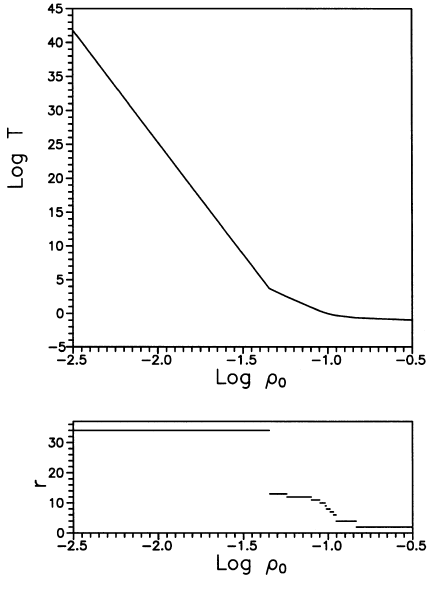
\includegraphics[scale=0.8]{Immagini1997.png}
	\caption{Andamento del "tempo di fuga" e dell'ordine ottimale $\tilde{r}_{opt}$ in funzione di $\rho_0$ (\cite{OTSA})} 
\end{figure}

Posto il parametro $\mu= 9.5387536 \cdot 10^{-4}$ corrispondente al caso Sole-Giove, le frequenze saranno $\omega_1 = 9.9675752552 \cdot 10^{-1}$ , $\omega_2= -8.0463875837 \cdot 10^{-2}$.
In tutta generalità, notando che la norma \ref{norm} dipende da $R_1$ e $R_2$, scegliamo $R_1 = 1= R_2$.
La figura \ref{Fig:T,rho} illustra l'andamento del "tempo di fuga" e di $\tilde{r}_{opt}$ in funzione del raggio $\rho_0$ del dominio iniziale.
Notiamo che il primo grafico è composto da segmenti rettilinei che diminuiscono la loro pendenza al diminuire di $\tilde{r}_{opt}$.
Infatti dalla \ref{eq:tau}, $$ LogT(\rho_0) \sim -mLog(\rho_0)+q $$ \\dove $m = \frac{1}{2\rho^{r+1}||\{I_j, H_{r+1}^{(r)})\}||_{R} } $ e $q = cost$ 

\subsection{Risultati per il problema di stabilità di L4}

In questa sezione, otterremo il dominio di stabilità di L4 per tempi dell'ordine dell'età dell'universo.

Dalla scelta delle unità di misura, $\omega=1$, la nostra unità di tempo è $\mathcal{T} = \frac{T_{Jup}}{2\pi}$ dove $T_{Jup}$ indica il periodo di rivoluzione di Giove attorno al Sole.
Con questa scala di tempo, discende che l'età dell'universo è $10^{10} \mathcal{T} $ a cui corrisponde $Log(\rho_0) = -1.536$ e, di conseguenza, $\rho_0 = 2.911 \cdot 10^{-2}$.

Osserviamo che $\rho_0$ è stato stimato attraverso l'analisi del problema in coordinate normali. Pertanto, per darne un significato fisico dovremo riportare il problema in coordinate polari.
Utilizzando l'inversa della \ref{cambiodicoor}, possiamo valutare la grandezza del dominio $$ \varDelta_{ \rho_0 R} = T_{\chi^{(r)}}^{-1} \varDelta_{ \rho_0 R}'  $$ \\dove $'$ indica il dominio nelle coordinate normali.
\\Dato che $\varDelta_{ \rho_0 R}'$ è prossimo ad un disco multidimensionale, ci si aspetta che anche la regione $\varDelta_{ \rho_0 R}$ lo sia. ?????? %chiedi spiegazione
 \\Il raggio $\rho$ nelle coordinate polari avrà la forma 
\begin{equation}
\label{stimarho}
\rho = \sqrt{( \rho_0^{2} - 2|I_j - I'_j| )}  
\end{equation}
\\dove $I_j$ e $I'_j$ sono le azioni, rispettivamente, in coordinate polari e normali.\\
Ricordando che $I_j = \frac{(x_j^2 + y_j^2)}{2}$ , $I'_j = \frac{({x'_j}^{2} + {y'_j})^{2}}{2}$, sappiamo dalla \ref{[proprietàT]} che $$I_j(x,y)|_{x=T_{\chi}^{-1} (x'_j, y'_j)} = (T_{\chi}^{-1}I_j)(x',y').$$
In più, il termine di destra della precedente equazione si può espandere in serie, con al primo termine proprio l'azione $I'_j$.
\\Quindi, $$ |I_j - I'_j|_{\rho_0 R} < {\rho_0^3 ||\varPhi_j^{(3)}||_R} + \cdots +{\rho_0^{\tilde{r}} ||\varPhi_j^{(\tilde{r})}||_R} .$$
Ancora una volta grazie alla \ref{[prop:limResto]}, la disguaglianza è verificata con $\rho_0$ minore o uguale a metà del raggio di convergenza della serie. In più, dati gli operatori $f_k$ e il valore precedente di $\rho_0$, $$|I_1-I'_1|_{\rho_0 R} \simeq 5.032 \cdot 10^{-5} < 0.110 I'_1 $$ e $$|I_2-I'_2|_{\rho_0 R} \simeq 1.834 \cdot 10^{-4} < 0.217 I'_2 .$$ 

Dalla \ref{stimarho}, concludiamo che il minimo dominio di stabilità si ha per $$\rho = \sqrt{( \rho_0^{2} - 2|I_2 - I'_2 |)} \simeq 2.192 \cdot 10^{-2} .$$
Dato, inoltre, $\rho_{Jup} = 1.718342 \cdot 10^{-1}$ ( la distanza L4-Giove ) osserviamo che il dominio di stabilità è circa 0.127 volte la distanza $\rho_{Jup}$.

\subsection{Confronto con gli asteroidi esistenti}

In modo da valutare l'accordo dei nostri risultati con gli asteroidi esistenti, useremo il catalogo degli asteroidi rilevati il 14/12/94, J.D.=2440700.5. \\Le coordinate riportate sul catalogo si sono dovute adattare al nostro problema. In breve, si è determinata la loro distanza da L4 proiettandola sul piano z=0, con coordinate $ x_1 $ , $ y_1 $ , $ x_2 $, $ y_2 $ che diagonalizzano l'hamiltoniana quadratica.

Il confronto è stato possibile ponendo $R_j = \sqrt{(x_j^2 + y_j^2)} $ ed è riportato in tabella (\ref{Fig:Tabdef1} e \ref{Fig:Tabdef2}). Notiamo, dalla definizione del dominio, che un determinato asteroide appartiene alla regione di stabilità sse $\rho_0 \geq 1$. Dunque, solo quattro asteroidi stanno nel dominio stimato; mentre la gran parte di essi si trova al di fuori da esso anche se solo di poco. Infatti, basterebbe migliorare $\rho_0$ di un fattore 10 per assicurarne la stabilità.

\begin{figure}[h]
	\label{Fig:Tabdef1}
	\centering
	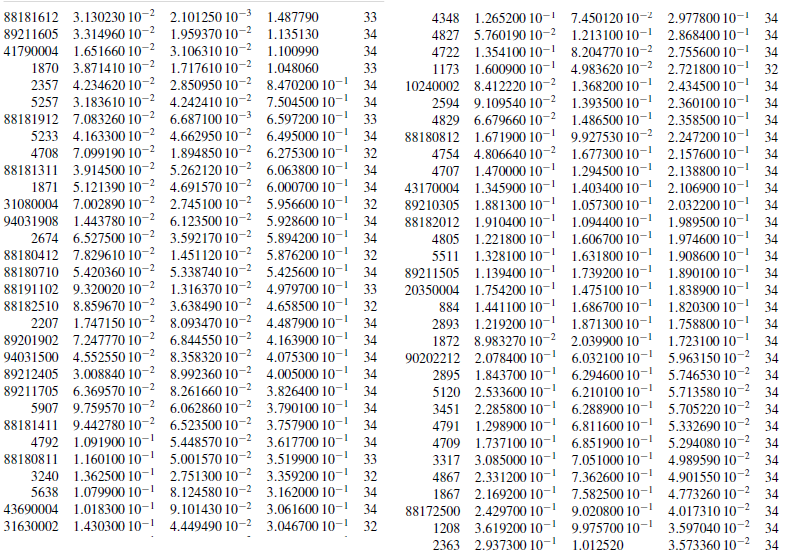
\includegraphics[scale=0.8]{Tabdef1.png}
	\caption{Tabella riassuntiva dei risultati analitici ottenuti(1).
	Nella prima colonna si trova il numero dell'asteroide; nella seconda e nella terza rispettivamente i valori di $R_1$ e $R_2$; nella terza il valore di $\rho_0$; mentre nell'ultima l'ordine ottimale dell'espansione in serie}
\end{figure}

\begin{figure}[h]
	\label{Fig:Tabdef2}
	\centering
	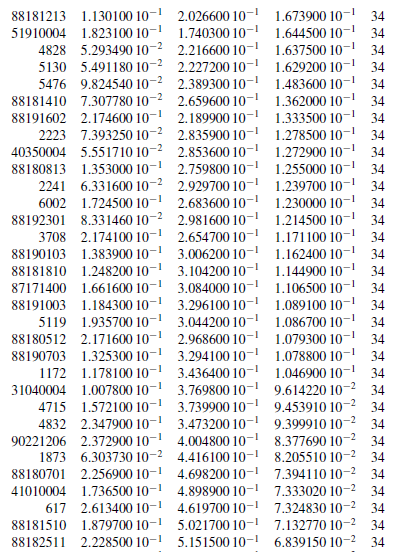
\includegraphics[scale=0.8]{Tabdef2.png}
	\caption{Tabella riassuntiva dei risultati analitici ottenuti(2).}
\end{figure}






\appendix

\chapter{Triangolo risolutivo della trasformata di Lie}

\begin{figure}[h]
	\label{Fig:TriangLie}
	\centering
	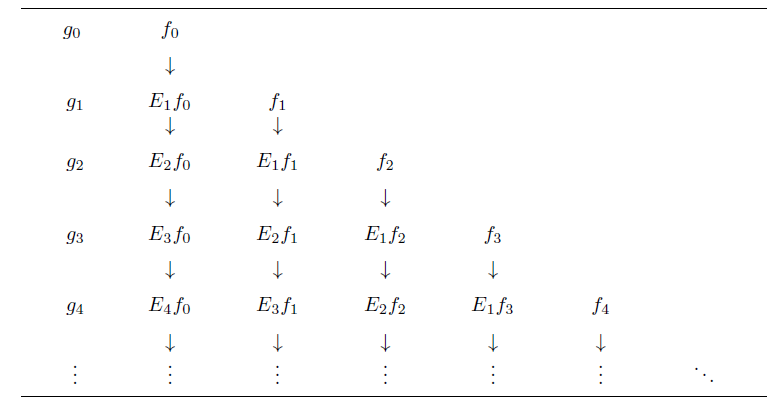
\includegraphics[scale=0.8]{TriangoloLie.png}
	\caption{Schema del processo risolutivo del sistema $g=T_{\chi}f$.} 
\end{figure}

In dettaglio, $f$, $g$ sono funzioni reali e il loro ordine k-esimo è identificato da $f_k$ , $g_k$.
In più, osserviamo che nelle "righe" si sono allineati i termini con dello stesso ordine; mentre in "colonna" si trovano i termini generati da $T_\chi \hspace{0.5mm} f_k $. Pertanto, la risoluzione del sistema di equazioni $g_k=T_{\chi}f_k$ avviene dalla prima riga, dalla quale si ricavano i termini k-1-esimi, per poi procedere verso il basso.




\chapter{Limitatezza delle funzioni in forma normale}
In questa parte, vogliamo dare un importante risultato per particolari polinomi omogenei $f$ e $\chi_s$. Infatti scelti $f$ e $\chi_s$ limitati, riusciremo a dare una stima della grandezza del "resto", della $f$ in forma normale e del raggio di convergenza della serie\cite{1989}:
\begin{prop}
	\label{[prop:limResto]}
	Siano $ \chi := \sum_{k \geq 3}\chi_k $, e $f = \sum_{k \geq 1} E_k$ con $f$,$E_k$,$\chi $,$\chi_ \in \varPi$. Assumiamo, inoltre, che $||\chi_k|| \leq a^{k-3} b$ e $||E_k|| \leq c^{k-1} d$, con $a,b,c,d \in \mathbb{R}_+$\texttt{\textbackslash}$\{0\}$.
	Ricordando che $T_\chi f= \sum_{k\geq 1} f_k  $ e introducendo il "resto" della forma $$\mathcal{R}^{(r)}= \sum_{k \geq r+1} f_k$$\\
	allora si ha \\\\ i) $||f_k|| \leq (3b + \frac{8}{3} a + c)^{k-1} d$\\
	ii) $T_\chi f$ è uniformemente convergente in qualsiasi disco multidimensionale
	$$D_R := \{(x,y) \in C^{2n}, |(x,y)| \leq R\} $$ con $R < R*$ dove $$R*=(3b + \frac{8}{3} a + c)^{-1}$$
	iii) $\mathcal{R}^{(r)}| \leq (\frac{R}{R*} )^r (1-\frac{R}{R*})^{-1} Rd $
\\\\dove $|.|$ per le funzioni indica il sup della funzione nel dominio.



	\end{prop}
\bibliography{bibliografia}
\bibliographystyle{plain} 




\end {document}

